% !TeX program = xelatex
% 中文研究初稿。Overleaf 中请选择 XeLaTeX 编译器。
% 本稿的统计数字以 FINAL_RESULTS_LOCK_CN.md（2026-08-28）为唯一来源。
\documentclass[preprint,12pt,authoryear]{elsarticle}

\usepackage[UTF8]{ctex}
\usepackage[a4paper,margin=2.5cm]{geometry}
\usepackage{booktabs}
\usepackage{threeparttable}
\usepackage{array}
\usepackage{multirow}
\usepackage{amsmath,amssymb}
\usepackage{graphicx}
\usepackage{float}
\usepackage{xcolor}
\usepackage{enumitem}
\usepackage{microtype}
\usepackage{tikz}
\usetikzlibrary{arrows.meta,positioning,fit,calc}
\usepackage[hidelinks]{hyperref}

\journal{Information Processing \& Management}
\biboptions{authoryear,round}

\newcommand{\todo}[1]{\textcolor{red!70!black}{[待作者补充：#1]}}
\newcommand{\pfwe}{p_{\mathrm{FWE}}}
\newcommand{\Ametric}{A2}
\renewcommand{\arraystretch}{1.18}

\begin{document}

\begin{frontmatter}

\title{超越单一视觉距离：算法化面部编辑中表面状态变化与编辑溯源的互补信息——行为与EEG证据}

\author[aff1]{\todo{作者姓名}}
\address[aff1]{\todo{作者单位、城市、国家及通讯邮箱}}

\begin{abstract}
算法化面部编辑的最终图像通常被压缩为单一视觉距离或质量分数，由此混淆了“输出变成什么样”与“系统怎样生成该输出”两类不可替代的信息。本研究重新分析一项由4个身份和FSlim、Eye、Mouth、Skin四类操作构成的被试内实验，区分输出状态信息与变换溯源信息。行为分析纳入30名参与者；按统一质量规则，EEG分析纳入28名参与者。双侧面颊局部表面外观变化指标A2具有预期构念负载，但在参与者分组交叉验证中仅使操作模型的$R^2$由$.145$提高至$.166$（$\Delta R^2=.021$），显示统计关联并不等同于较高的信息效用。变换溯源方面，Skin在350--600 ms中央--顶叶窗口呈负向电位差异（$\pfwe=.0154$），Eye在600--1000 ms窗口呈正向电位差异（$\pfwe=.0063$）；两项结果均通过28次留一参与者检验，并在四种身份遗漏版本中保持方向一致。连续A2 EEG效应、ERP--评价关联及ERP评分增量预测均未获支持。结果表明，输出状态和变换溯源应作为互补记录被保留：前者为用户评价提供有限增量信息，后者提供条件相关的时间敏感证据；二者不能合并为统一神经级联。
\end{abstract}

\begin{keyword}
数字面部编辑 \sep 信息表征 \sep 数据溯源 \sep 用户评价 \sep EEG \sep 事件相关电位 \sep 信息效用
\end{keyword}

\end{frontmatter}

\section{引言}

算法化图像系统把一系列变换压缩为可见的最终输出。若信息系统只保存最终图像或一个总体视觉距离，用户和审计者便难以区分两类问题：输出状态究竟改变了多少，以及哪些系统活动产生了这种变化。数据溯源研究强调，数据实体应与产生它们的活动保持可追踪联系；人本人工智能研究同样要求系统在适当时点呈现其能力、行为和结果来源\citep{MoreauMissier2013,Simmhan2005,Amershi2019,Miller2019}。因此，算法化视觉信息的充分表征不只是提高图像描述精度，也涉及是否保留了变换来源。

面部编辑为这一问题提供了一个边界清晰的场景。一次编辑可以改变轮廓、眼部、口部或皮肤表面；吸引力、自然度、可信度与自我呈现也不必同向变化\citep{Appel2023,Hong2020,Javornik2022,Dijkslag2024}。将复杂输出压缩为“是否美化”或单一距离，会同时丢失局部变化幅度与编辑来源。本文据此区分两类互补而非上下级的信息内容：\emph{输出状态信息}描述最终图像相对原图的表面变化；\emph{变换溯源信息}记录系统执行了何种编辑操作。前者回答“变成了什么样”，后者回答“怎样变成这样”。

这一区分还要求分别评价统计关联和信息效用。一个计算指标可能在大样本的样本内模型中高度显著，却只对未见参与者提供很小的预测增量；构念效度、样本外效用与神经时间对应因此不是同一个证据标准\citep{Shmueli2010,WangStrong1996}. 对面孔图像而言，局部特征、特征间配置和表面反射信息本来也具有不同作用\citep{TanakaFarah1993,Maurer2002,Russell2007,TanakaSimonyi2016}。本研究使用局部表面变化指标量化输出状态，并用FSlim、Eye、Mouth和Skin标签保存变换溯源，检验二者是否提供不可替代的信息。

EEG在这里是人类时间加工的证据通道，而不是系统表征本身。既有研究表明，面孔与吸引力信息可影响早期活动，也可在约300 ms以后伴随更持续的评价相关电位变化\citep{Bentin1996,Schacht2008,ZhangDeng2012,Revers2023}。然而，窗口内电压差异并不能自动命名为心理阶段，更不能仅凭先后顺序建立“图像指标$\rightarrow$EEG$\rightarrow$评价”的因果路径。本文因此把EEG用于定位条件相关的时间范围，并直接检验连续指标--EEG、EEG--评价及预测增量是否成立。

本研究对既有数据进行联合多重校正的重新分析，不改变原实验、参与者或刺激。具体研究问题为：

\begin{enumerate}[label=\textbf{RQ\arabic*.},leftmargin=2.4em]
  \item 局部表面外观变化指标A2是否主要响应Skin操作，并与几何变化、身份距离和错位保持区分？
  \item 在变换溯源标签之外，A2能否为Beauty和Naturalness评价提供未见参与者上的增量解释？
  \item 四类编辑操作是否在事先锁定的中央--顶叶时间窗中表现出操作相关电位差异？
  \item 这些差异是否对参与者与身份遗漏保持稳定，并能否与评价形成个体层关联或预测增量？
\end{enumerate}

本研究聚焦两项贡献。第一是\emph{表征贡献}：把输出状态与变换溯源定义为算法化视觉信息的互补内容，而不是把二者压缩为单一美化距离。第二是\emph{评价原则贡献}：把构念效度、未见参与者上的信息效用和神经时间对应作为三个不同门槛。统一样本、多重校正和零结果报告是实现这两个贡献的方法保障，而不是额外的理论主张。

\section{理论框架}

\subsection{输出状态与变换溯源的互补表征}

输出状态指标回答“最终图像的局部表面改变了多少”。本研究以A2表示相对于同一身份原始图像的双侧面颊色彩、亮度和纹理变化。变换溯源变量回答“系统执行了哪一种编辑”。FSlim、Eye、Mouth和Skin因而保存编辑活动的来源。两类信息可能相关，例如Skin通常带来更大的表面变化；但它们不可互相替代，因为操作标签不能精确决定每张图像的实际变化幅度，连续距离也不能恢复编辑区域和操作类型。规范化的数据记录同样强调结果实体、生成活动及其属性的共同保存\citep{MoreauMissier2013,Mitchell2019,Gebru2021}。

图\ref{fig:framework}把系统层的信息表征、人类观察反应和未获支持的连接分开。A2对评价具有有限参与者外增量；操作类别在评价和预定义窗口EEG中均有条件差异。连续A2 EEG追踪以及EEG个体差异对评价的关联或增量预测未获支持。因此，这是两个互补信息内容与两种观察结果之间的条件关联，不是神经中介模型。

\begin{figure}[H]
\centering
\begin{tikzpicture}[
  node distance=8mm and 13mm,
  head/.style={font=\bfseries,align=center},
  box/.style={draw,rounded corners,align=center,minimum width=39mm,minimum height=13mm,fill=blue!4},
  ebox/.style={draw,rounded corners,align=center,minimum width=39mm,minimum height=13mm,fill=orange!7},
  nbox/.style={draw,dashed,rounded corners,align=center,minimum width=39mm,minimum height=13mm,fill=gray!6},
  arr/.style={-{Latex[length=2.3mm]},thick},
  fail/.style={-{Latex[length=2.3mm]},thick,dashed,gray}
]
\node[head] (h1) {信息表征};
\node[head,right=28mm of h1] (h2) {观察反应};
\node[head,right=28mm of h2] (h3) {未获支持的连接};
\node[box,below=of h1] (a2) {输出状态\\局部表面变化A2};
\node[box,below=of a2] (op) {变换溯源\\编辑操作与区域};
\node[ebox,below=of h2] (beh) {用户评价\\Beauty/Naturalness};
\node[ebox,below=of beh] (erp) {时间敏感EEG\\窗口电位差异};
\node[nbox,below=of h3] (a2eeg) {A2 $\rightarrow$ EEG\\联合校正后为零};
\node[nbox,below=of a2eeg] (eegbeh) {EEG $\rightarrow$ 评价\\关联与增量预测为零};
\draw[arr,blue!70!black] (a2) -- node[above,font=\scriptsize]{有限增量} (beh);
\draw[arr,blue!70!black] (op) -- (beh);
\draw[arr,orange!80!black] (op) -- (erp);
\draw[fail] (a2) -- (a2eeg);
\draw[fail] (erp) -- (eegbeh);
\end{tikzpicture}
\caption{互补信息表征、观察反应及当前证据边界。实线为当前刺激集内的条件关联；虚线框为联合校正后未获支持的连接，均不表示因果关系。}
\label{fig:framework}
\end{figure}

\subsection{评价加工的时间范围与可检验边界}

既有ERP研究为结果解释提供宽泛的时间参照：0--200 ms常与基础视觉和面孔结构编码相关，200--350 ms可能包含特征选择与初步价值区分，350--600 ms可能涉及后知觉的评价整合或表征比较，600--1000 ms可能包含持续注意、评价精加工与反应准备\citep{Schacht2008,Revers2023,Han2022}。这些是相互重叠的解释范围，而不是离散加工阶段。当前分析只检验两个既有特征窗口的平均电压，完整0--1000 ms联合簇检验又未确定显著簇。因此，Skin和Eye结果只能被定位于中晚期和晚期时间范围，不能证明完整级联或精确阶段边界。

\section{方法}

\subsection{参与者与分析样本}

原实验招募30名大学生，其中女性15名、男性15名，均报告视力正常或矫正正常。行为分析保留全部30名参与者。EEG样本采用统一且不依据显著性选择的质量规则：s5不在默认有效EEG名单中；s18虽然保留16个因子格，但13个格低于每格8个有效试次的门槛，因而排除。主EEG样本为28人（s1--s4、s6--s17、s19--s30）。每名参与者在窗口模型中贡献196--384个有效编辑图像试次，总计9,626个试次；28人均覆盖全部16个因子格，设计矩阵满秩。参与者是统计推断与置换单位，试次数不被当作样本量。\todo{按期刊要求补充伦理审批编号和知情同意表述；本稿暂不处理伦理内容。}

\subsection{刺激、编辑操作与实验流程}

刺激包含4个陌生、中性表情身份（F\_1、F\_2、M\_1和M\_2；两女两男）。FSlim、Eye、Mouth和Skin分别设置两个水平，形成被试内$2\times2\times2\times2$完全交叉设计。Eye和Mouth操纵局部特征大小，FSlim操纵面部轮廓，Skin操纵皮肤美白和平滑。每个身份产生16张编辑图像及1张未编辑基线，共68张核心图像。64张编辑图像是4个身份的重复变体，而不是64个独立身份刺激。

每名参与者在正式任务中观看每张核心图像6次，共408个任务试次；另有60个1-back注意检查试次，实验分为4个区组。每个试次首先呈现2,000 ms中央注视点，随后呈现500 ms面孔，再记录Beauty和Naturalness两个7级评价字段，试次间隔为500--800 ms抖动。A2和主行为模型使用64张编辑图像对应的记录；未编辑基线用于计算同身份视觉变化。\todo{核对并补入最终量表端点文字、屏幕尺寸、观看距离和按键映射。}

\subsection{局部表面外观变化指标A2}

A2是本次事后重新分析中开发的替代指标，并非原实验预注册变量。其公式、面颊区域、三个成分、等权权重与标准化方式均在评估本次行为和EEG关联之前写入规格并锁定；锁定后没有并行测试多个A2实现再按显著性选择。首先利用5个面部标志点，把每张编辑图像通过相似变换对齐至同身份原图。随后仅在双侧面颊区域计算三个原始差异量：

\begin{enumerate}[label=(\arabic*),leftmargin=2em]
  \item Lab颜色空间$a/b$二维直方图的Jensen--Shannon散度；
  \item 平均绝对$L^*$亮度变化；
  \item 四方向Gabor滤波纹理响应变化。
\end{enumerate}

对第$j$张图像的第$k$个成分$d_{jk}$进行均方根缩放，三个成分等权平均：
\begin{equation}
  A2_j=\frac{1}{3}\sum_{k=1}^{3}
  \frac{d_{jk}}{\sqrt{J^{-1}\sum_{j=1}^{J}d_{jk}^{2}}}.
  \label{eq:a2}
\end{equation}
该方案不复用原A的皮肤分割、SSIM、LBP或边缘成分。A2只代表双侧面颊区域的局部表面外观变化，不代表整体面部外观或一般图像质量。构念检查包括A与A2的Pearson和Spearman相关、Skin对A2的效应、FSlim交叉负载、几何对齐残差、A2与复现几何指标$G_{new}$及身份距离$I$的相关，以及身份遗漏敏感性。$G_{new}$使用锁定MediaPipe环境重新检测全部68张图像的468点并沿用既有七成分公式；$I$为SFace身份嵌入相对于同身份原图的余弦距离。由于$G_{new}$与旧G的一致性不足，详细结果只进入补充测量审计，主文不以G形成理论主张\citep{Lugaresi2019}。

\subsection{EEG采集与预处理}

EEG使用Neuroscan SynAmps 2放大器、64导电极帽和Curry 8软件，以1,000 Hz采样。恢复的原始流程为：通过EEGLAB的\texttt{loadcurry}导入Curry文件；使用\texttt{pop\_eegfiltnew}进行0.1--30 Hz FIR滤波；在可用时条件性执行50 Hz CleanLine；坏道处理优先采用\texttt{clean\_rawdata}（平线5 s、通道相关$.80$、线噪阈值4，关闭burst/window拒绝），否则使用峰度阈值5；平均参考；在连续数据上运行extended runica；使用ICLabel并仅在Eye类别概率$\geq .90$时移除眼动成分；依据事件码配对提取正式试次；以$-200$至1,000 ms分段并以$-200$至0 ms校正基线；任一保留通道超过$\pm120\ \mu$V的epoch被剔除。

分析就绪数据包含61个保留通道、平均参考元数据、ICA矩阵、ICLabel分类概率、清洁通道掩码和约$-200$至1,000 ms的epoch。CleanLine是否对每名参与者实际运行、每名参与者采用哪一种坏道分支，以及完整的成分和epoch拒绝编号无法逐人恢复；论文因此将其报告为协议层面复原，而不声称逐参与者完全可执行重现。

\subsection{行为统计分析}

行为长数据包含30名参与者的23,040条维度评价观测。Beauty与Naturalness在同一混合模型中联合分析，是因为二者属于同一实验中的相关评价结果，联合建模可以把它们置于一个一致的推断族中，并直接检验A2效应是否因评价维度而异；这不是把两个评分字段当作独立参与者来扩大样本量。模型同时包含评分维度、四个编辑操作、A2及其与评分维度的交互，并控制身份；随机部分包含参与者截距与评分维度随机斜率。A2的增量拟合通过仅含操作因子的Factor模型与Factor+A2模型的似然比、AIC和BIC比较。预测层面采用按参与者分组的5折交叉验证，确保同一参与者的记录不会同时进入训练集和测试集。该设计只检验未见参与者预测；同一批图像仍由多人重复评价，因而不检验未见身份或新刺激预测。

为了与EEG样本匹配，另在28人样本中逐参与者估计Beauty和Naturalness的FSlim、Eye、Mouth和Skin系数，同时控制标准化试次顺序和身份固定效应。8个操作$\times$评价检验使用10,000次参与者符号翻转的最大-$|t|$校正。操作系数表示编码水平1减水平0；在最终核实量表和操作方向前，不把系数符号直接改写为“改善”或“损害”。

\subsection{预定义窗口EEG分析}

窗口分析使用中央--顶叶ROI：CPz、Pz、CP1、CP2、P1和P2。350--600 ms与600--1000 ms窗口来自Stage 2既有EEG特征提取方案，并在当前四操作最大-$|t|$检验及结果查看前写入特征清单；它们不是根据本次Skin或Eye统计量截取的。两个宽窗口分别覆盖既有文献中的后知觉中晚期评价范围与持续晚期活动范围\citep{Schacht2008,Revers2023,Han2022}，但不被视为离散心理阶段。对每名参与者和每个窗口，在单试次层面同时估计FSlim、Eye、Mouth和Skin，并控制标准化试次顺序和身份固定效应。这样得到每名参与者的8个系数（4个操作$\times$2个窗口）。群体推断采用10,000次参与者层符号翻转；每次置换使用同一个符号作用于该参与者的完整8系数向量，以8项中最大绝对$t$值构造familywise零分布。随机种子为20261828。除非另有说明，本文分析均为事后探索性但控制多重性；没有任何分析被称为前瞻性预注册确认性检验。

\subsection{稳健性、完整时程与跨层边界分析}

对通过校正的窗口效应执行28次留一参与者分析，每次重新进行相同的8项最大-$|t|$校正。身份敏感性通过依次排除F\_1、F\_2、M\_1和M\_2后重新估计模型实现。由于只有4个身份，这些分析只能识别单一身份影响，不能支持新身份总体推断。

完整时程边界分析把FSlim、Eye、Mouth、Skin和Surface-minus-Structural五个信号同时纳入0--1000 ms联合最大簇校正，簇形成阈值为双侧逐点$p<.05$，簇质量为连续时间点绝对$t$值之和，置换单位为参与者。连续视觉信息模型同时拟合$G_{new}$/A2/$I$并在指标$\times$时间范围内联合校正。跨层检验包括参与者层操作ERP系数与相应行为系数的相关，以及嵌套留一参与者评分预测中ERP的增量价值\citep{MarisOostenveld2007}。MVPA、RSA与详细G复现属于补充边界审计，不用于从多个分析路线中挑选有利结果。

\section{结果}

\subsection{样本与质量控制}

30名参与者进入行为分析。统一EEG样本排除s5和s18后为28人，共有9,626个有效编辑图像正式试次；每名参与者保留196--384个试次，均覆盖16个因子格且设计矩阵满秩。N=29版本仅作为样本敏感性分析，不用于根据显著性选择主样本。

\subsection{A2的构念效度}

A2与原A的Pearson相关为$.6189$，Spearman相关为$.7573$，说明二者共享表面外观变化信息，但并非同一实现。Skin对A2的效应显著（$\beta=1.6466$，$SE=.1318$，$p=8.40\times10^{-36}$），而FSlim交叉负载不显著（$\beta=.0319$，$p=.8492$）。几何对齐残差与A2无关（$\beta=.0059$，$p=.9763$）。A2与$G_{new}$和$I$的相关分别为$-.0521$和$.0720$。身份遗漏分析中，Skin系数为1.2225--1.9666，四个版本方向均为正且$p\leq2.10\times10^{-21}$。这些结果支持A2作为当前刺激集内相对独立的\emph{局部面颊表面变化指标}，但不支持整体外观测量或新身份总体泛化（图\ref{fig:a2validity}）。

\begin{table}[H]
\centering
\caption{A2的主要构念检验}
\label{tab:a2validity}
\begin{threeparttable}
\begin{tabular}{p{5.4cm}rrl}
\toprule
检验 & 估计值 & $p$值 & 解释 \\
\midrule
原A与A2（Pearson） & $r=.6189$ & --- & 中等一致性 \\
原A与A2（Spearman） & $\rho=.7573$ & --- & 排序一致性较高 \\
Skin$\rightarrow$A2 & $\beta=1.6466$ & $8.40\times10^{-36}$ & 预期构念效应 \\
FSlim$\rightarrow$A2 & $\beta=.0319$ & $.8492$ & 无几何操作交叉负载 \\
对齐残差$\rightarrow$A2 & $\beta=.0059$ & $.9763$ & 无明显错位影响 \\
A2与$G_{new}$ & $r=-.0521$ & --- & 基本区分 \\
A2与$I$ & $r=.0720$ & --- & 基本区分 \\
\bottomrule
\end{tabular}
\begin{tablenotes}\small
\item 注：相关和回归均基于冻结A2定义；未在多个A2方案间按显著性选择。
\end{tablenotes}
\end{threeparttable}
\end{table}

\begin{figure}[H]
\centering
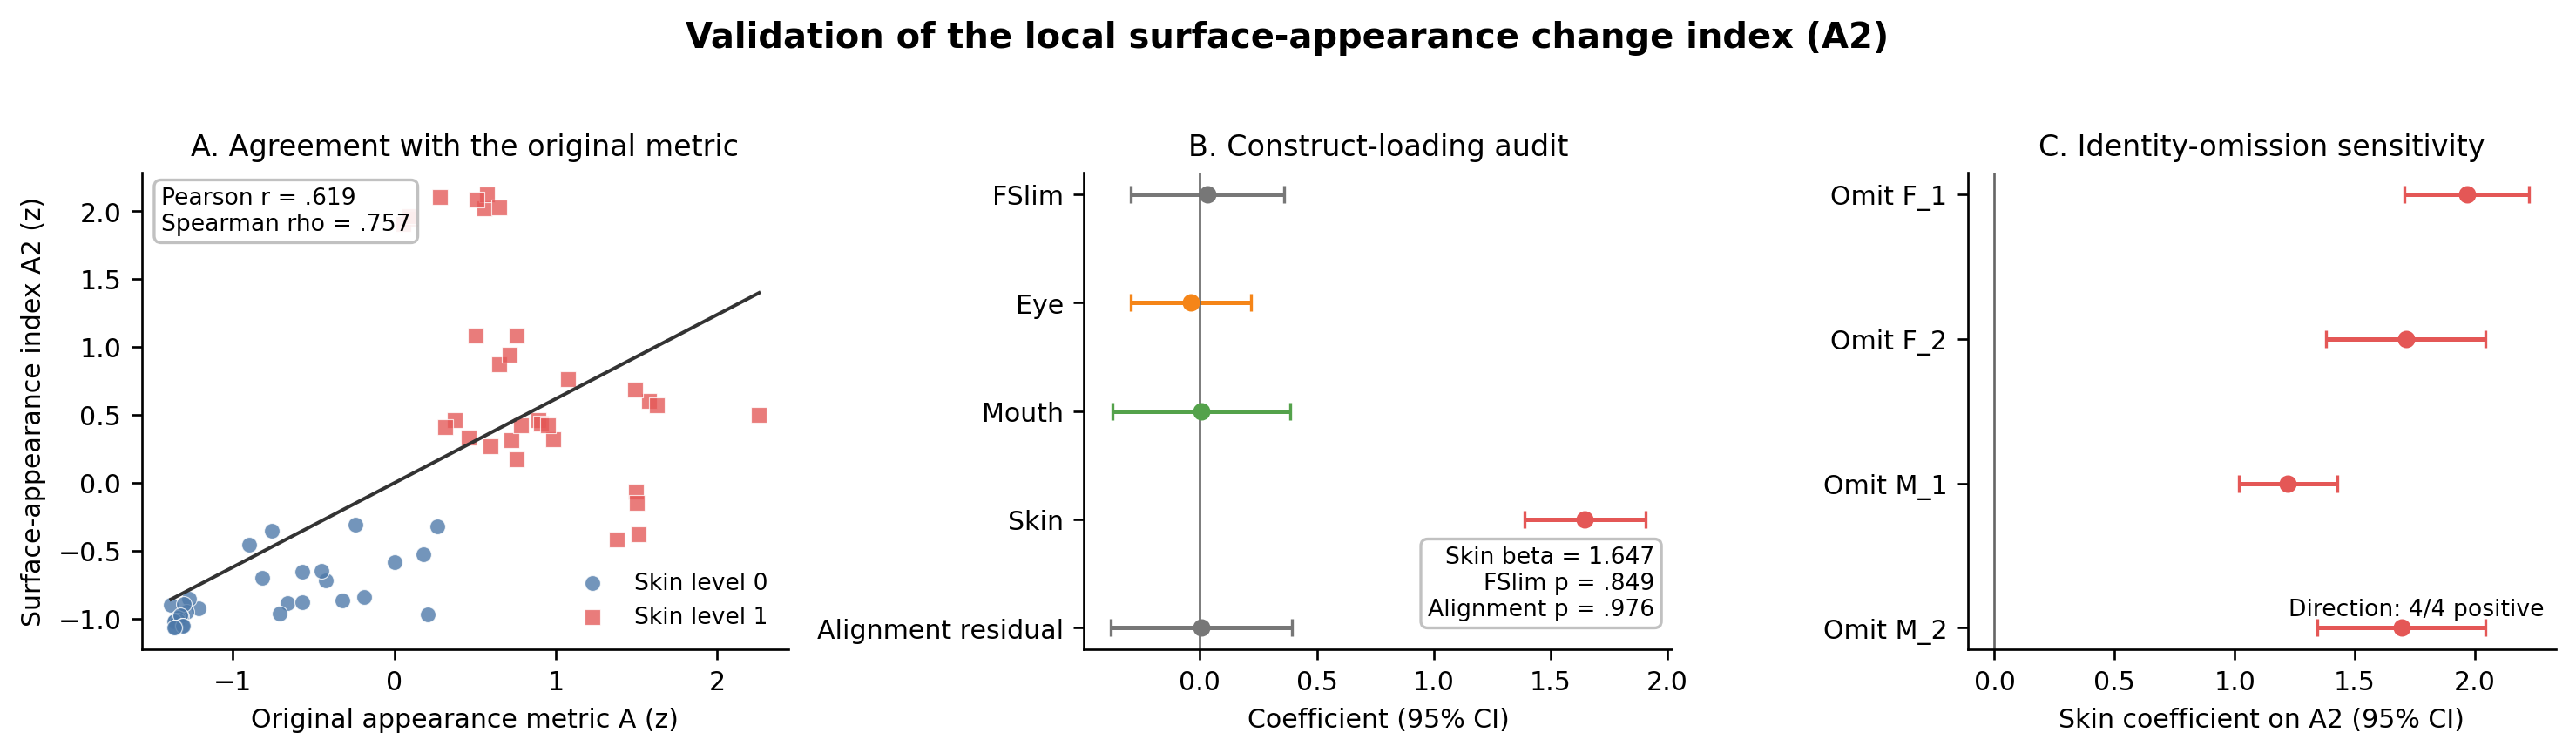
\includegraphics[width=\textwidth]{figures/Figure_2_A2_construct_validation.png}
\caption{A2构念验证。A：原A与冻结A2按Skin条件的关系；B：Skin预期负载、FSlim交叉负载和对齐残差检验；C：身份遗漏敏感性。图C仅检验单一身份是否主导结果，不是新身份泛化检验。误差线为95\%置信区间。}
\label{fig:a2validity}
\end{figure}

\subsection{A2对行为评价的有限增量价值}

相对于Factor模型，Factor+A2模型显著改善样本内拟合，似然比$\chi^2(2)=700.1909$，$p=9.03\times10^{-153}$；$\Delta\mathrm{AIC}=-696.19$，$\Delta\mathrm{BIC}=-680.10$。Factor+A2模型中，A2主效应为$\beta=.2977$（$SE=.0209$，$z=14.24$，$p=5.06\times10^{-46}$），Beauty维度$\times$A2交互为$\beta=-.6896$（$SE=.0260$，$z=-26.51$，$p=7.76\times10^{-155}$）。这些极小$p$值反映观测量较多时的稳定统计关联，不能单独证明A2具有较高的信息效用。

参与者分组5折交叉验证结果见表\ref{tab:cv}与图\ref{fig:cvfolds}。Factor+A2模型的$R^2=.1657$，相对于Factor模型提高$.0211$；RMSE降低$.0155$，MAE降低$.0127$。五折的$\Delta R^2$均为正，范围为$.0183$--$.0265$，说明小幅增量并非由单一折产生。统计关联与信息效用在这里明显分离：A2提供可检测但有限的未见参与者增量，而不是高精度、未见图像或新身份预测器。

\begin{table}[H]
\centering
\caption{按参与者分组的5折交叉验证}
\label{tab:cv}
\begin{tabular}{lrrr}
\toprule
模型 & RMSE & MAE & $R^2$ \\
\midrule
A2 only & 1.2797 & .9912 & .0985 \\
Factor & 1.2465 & .9692 & .1446 \\
Factor + A2 & \textbf{1.2310} & \textbf{.9564} & \textbf{.1657} \\
\bottomrule
\end{tabular}
\end{table}

\begin{figure}[H]
\centering
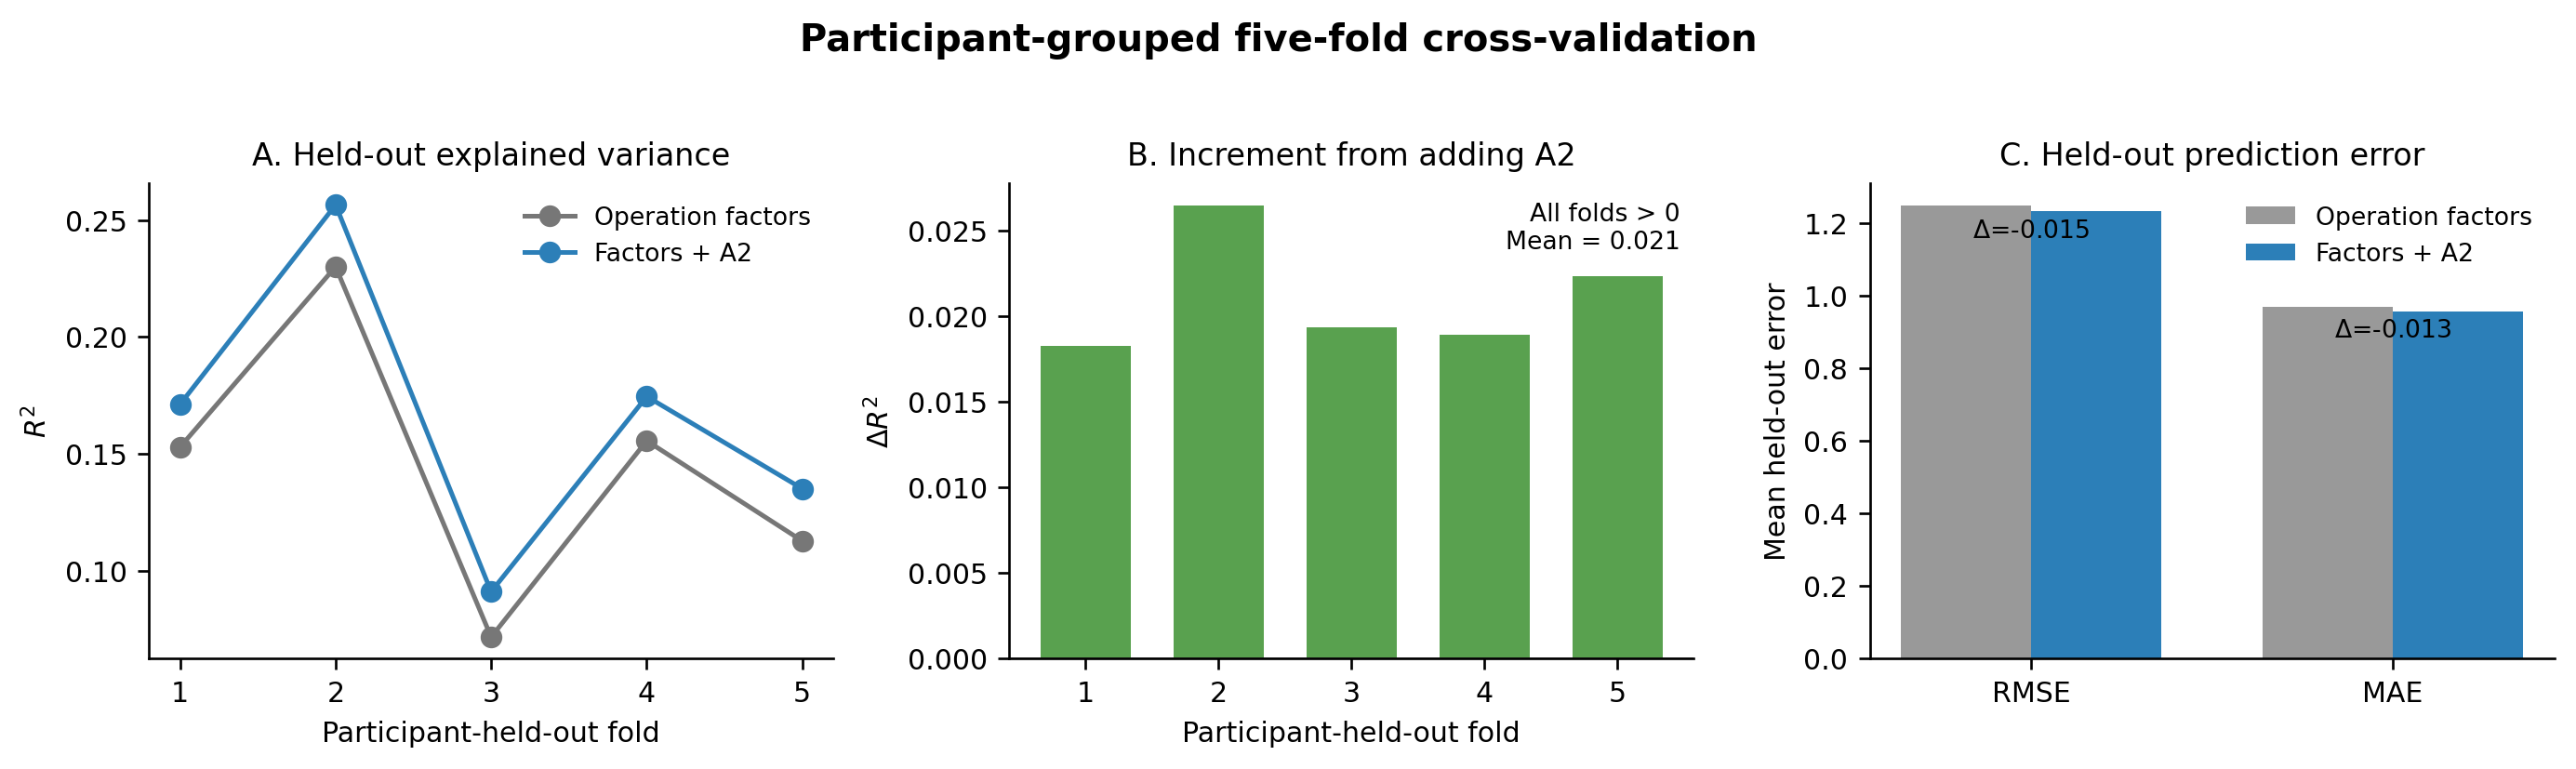
\includegraphics[width=\textwidth]{figures/Figure_3_behavior_cv_folds.png}
\caption{按参与者分组的五折交叉验证。每折训练集和测试集的参与者不重叠；同一组图像仍在不同参与者间重复，因此该结果仅表示未见参与者预测，不表示未见刺激或新身份泛化。}
\label{fig:cvfolds}
\end{figure}

\subsection{操作层行为效应}

在匹配的28人样本中，FSlim、Eye和Skin对两个评价字段的操作系数均通过8项最大-$|t|$校正，Mouth未通过校正（表\ref{tab:behavior}）。这些结果说明操作来源在两个评价维度中均保留了可检测信息，但系数方向只表示编码水平1与0之差，不直接等同于更美、更自然或更不自然。

\begin{table}[H]
\centering
\caption{匹配EEG样本中的操作层行为结果}
\label{tab:behavior}
\begin{threeparttable}
\begin{tabular}{llrrrr}
\toprule
评价 & 操作 & $\beta$ & 95\% CI & $t(27)$ & $\pfwe$ \\
\midrule
Beauty & FSlim & $-.1835$ & $[-.2661,-.1009]$ & $-4.558$ & $.00030$ \\
Beauty & Eye   & $-.4428$ & $[-.6207,-.2650]$ & $-5.109$ & $.00020$ \\
Beauty & Mouth & \multicolumn{3}{c}{校正后不显著} \\
Beauty & Skin  & $-.1658$ & $[-.2448,-.0869]$ & $-4.309$ & $.00070$ \\
Naturalness & FSlim & $.2283$ & $[.1446,.3120]$ & $5.598$ & $.00020$ \\
Naturalness & Eye   & $.7157$ & $[.4687,.9626]$ & $5.947$ & $.00010$ \\
Naturalness & Mouth & \multicolumn{3}{c}{校正后不显著} \\
Naturalness & Skin  & $.4093$ & $[.2600,.5586]$ & $5.625$ & $.00020$ \\
\bottomrule
\end{tabular}
\begin{tablenotes}\small
\item 注：Mouth的$\pfwe$分别为$.1428$和$.4652$。校正族包含2个评价字段$\times$4个操作。
\end{tablenotes}
\end{threeparttable}
\end{table}

\subsection{预定义窗口的操作敏感型ERP结果}

8项联合校正中有两项通过familywise门槛（表\ref{tab:eegall}）。Skin在350--600 ms产生中央--顶叶负向差异，$\beta=-.2789\ \mu$V，95\% CI $[-.4507,-.1071]$，$t(27)=-3.330$，$\pfwe=.0154$，$d_z=-.629$。Eye在600--1000 ms产生正向差异，$\beta=.2884\ \mu$V，95\% CI $[.1270,.4498]$，$t(27)=3.666$，$\pfwe=.0063$，$d_z=.693$。其余6项均未通过同一校正。Mouth在350--600 ms的未校正$p=.0177$，但$\pfwe=.1101$，因此不作为显著结果解释。

\begin{table}[H]
\centering
\caption{两个预定义中央--顶叶窗口中的完整8项EEG结果}
\label{tab:eegall}
\begin{threeparttable}
\begin{tabular}{llrrrr}
\toprule
窗口 & 操作 & $\beta$ ($\mu$V) & 95\% CI & $t(27)$ & $\pfwe$ \\
\midrule
350--600 ms & FSlim & $.0429$ & $[-.1081,.1940]$ & $.583$ & $.9969$ \\
350--600 ms & Eye   & $.0277$ & $[-.1404,.1959]$ & $.339$ & $1.0000$ \\
350--600 ms & Mouth & $-.1866$ & $[-.3382,-.0351]$ & $-2.527$ & $.1101$ \\
350--600 ms & Skin  & $\mathbf{-.2789}$ & $\mathbf{[-.4507,-.1071]}$ & $\mathbf{-3.330}$ & $\mathbf{.0154}$ \\
600--1000 ms & FSlim & $.0713$ & $[-.0846,.2272]$ & $.939$ & $.9428$ \\
600--1000 ms & Eye   & $\mathbf{.2884}$ & $\mathbf{[.1270,.4498]}$ & $\mathbf{3.666}$ & $\mathbf{.0063}$ \\
600--1000 ms & Mouth & $-.0772$ & $[-.2354,.0809]$ & $-1.002$ & $.9229$ \\
600--1000 ms & Skin  & $-.1702$ & $[-.3514,.0110]$ & $-1.927$ & $.3585$ \\
\bottomrule
\end{tabular}
\begin{tablenotes}\small
\item 注：10,000次参与者符号翻转；$\pfwe$为8项最大-$|t|$校正。粗体表示通过$.05$门槛。
\end{tablenotes}
\end{threeparttable}
\end{table}

\begin{figure}[H]
\centering
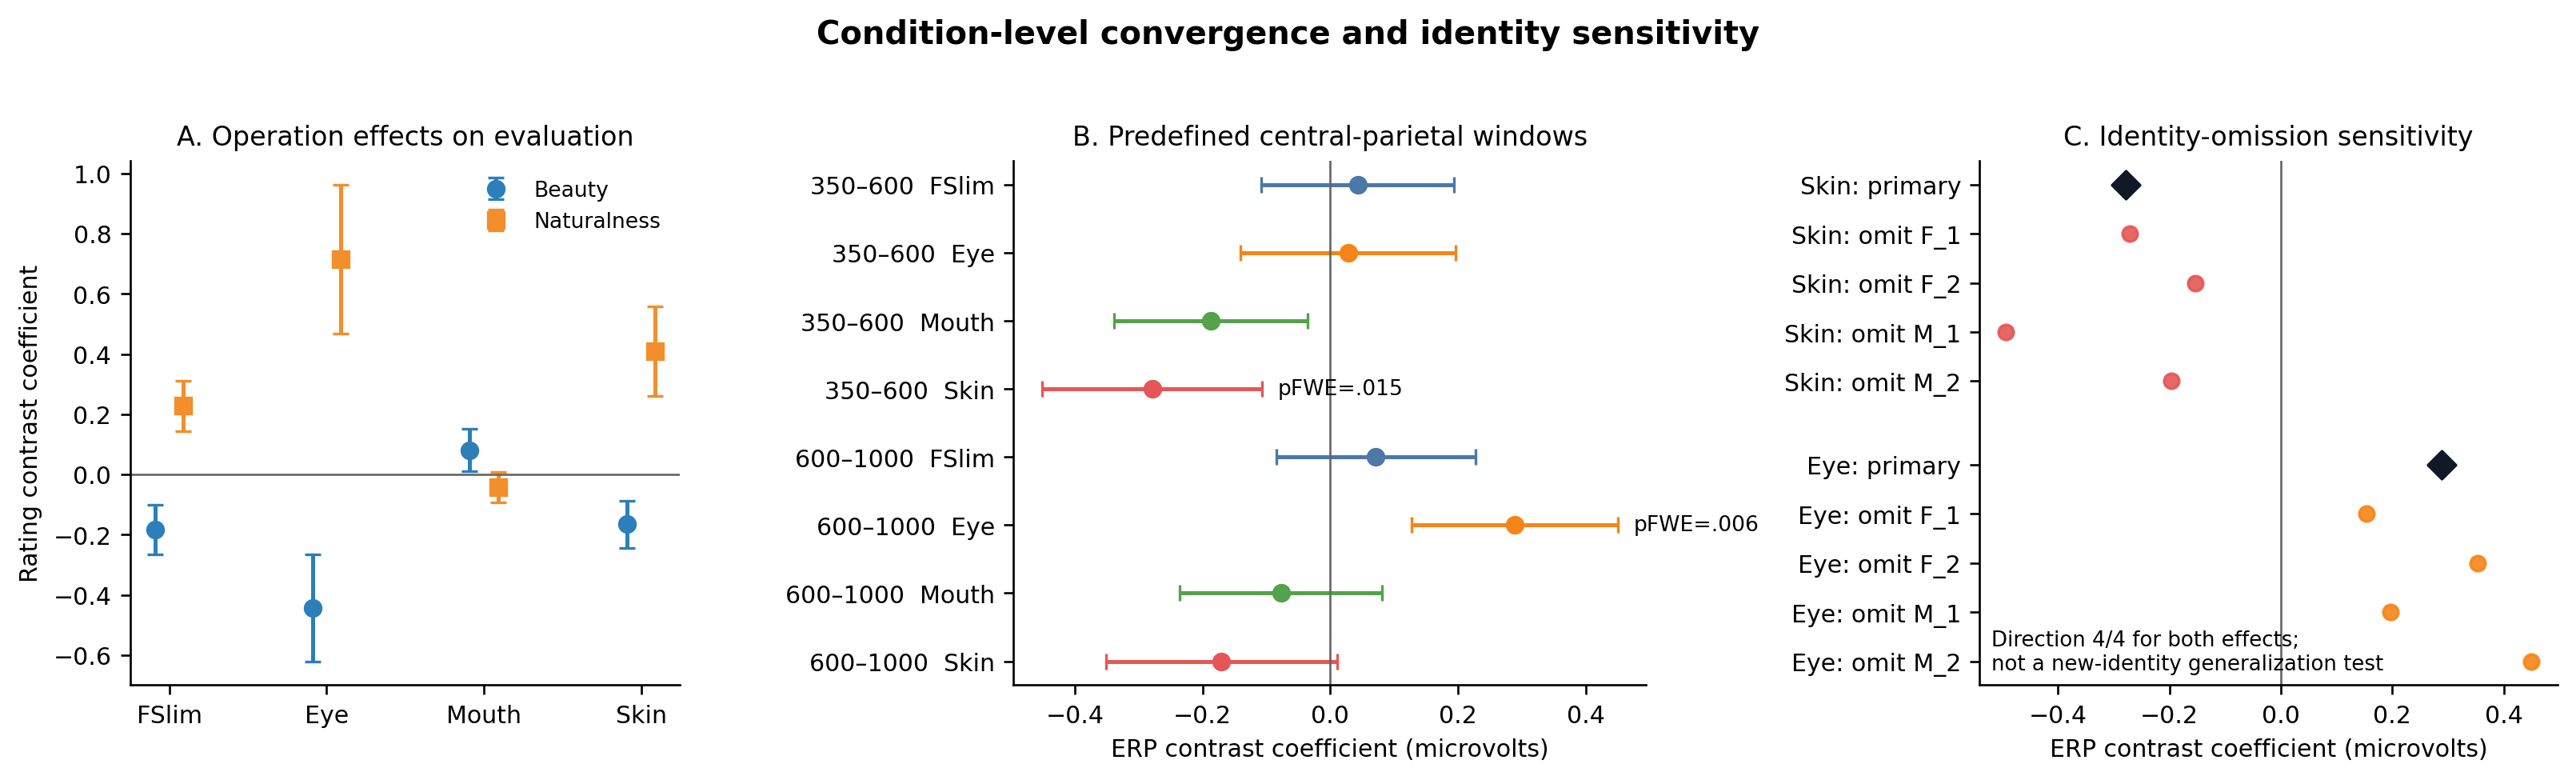
\includegraphics[width=\textwidth]{figures/Figure_4_operation_evidence.png}
\caption{变换溯源的行为与EEG证据。A：操作对两个评价字段的系数；B：两个锁定中央--顶叶窗口中的完整8项操作系数；C：身份遗漏敏感性。图C不构成新身份泛化检验。误差线为95\%置信区间。}
\label{fig:operation}
\end{figure}

\subsection{参与者与身份敏感性}

Skin 350--600 ms效应在28次留一参与者分析中28/28仍通过相同8项最大-$|t|$校正，方向一致率为100\%，最不利版本$\pfwe=.0337$。Eye 600--1000 ms同样在28/28版本中通过校正，方向一致率100\%，最不利版本$\pfwe=.0143$。因此，两项固定窗口结果均不由单一参与者决定。

依次排除F\_1、F\_2、M\_1和M\_2时，Skin 350--600 ms的$\beta$分别为$-.2705$、$-.1536$、$-.4931$和$-.1970\ \mu$V，四个版本方向一致；Eye 600--1000 ms的$\beta$分别为$.1535$、$.3531$、$.1974$和$.4492\ \mu$V，同样方向一致。由于只有部分版本通过8项校正，这一结果只能称为身份遗漏下的方向稳定，不能称为跨身份显著复现或新身份泛化。

\begin{figure}[H]
\centering
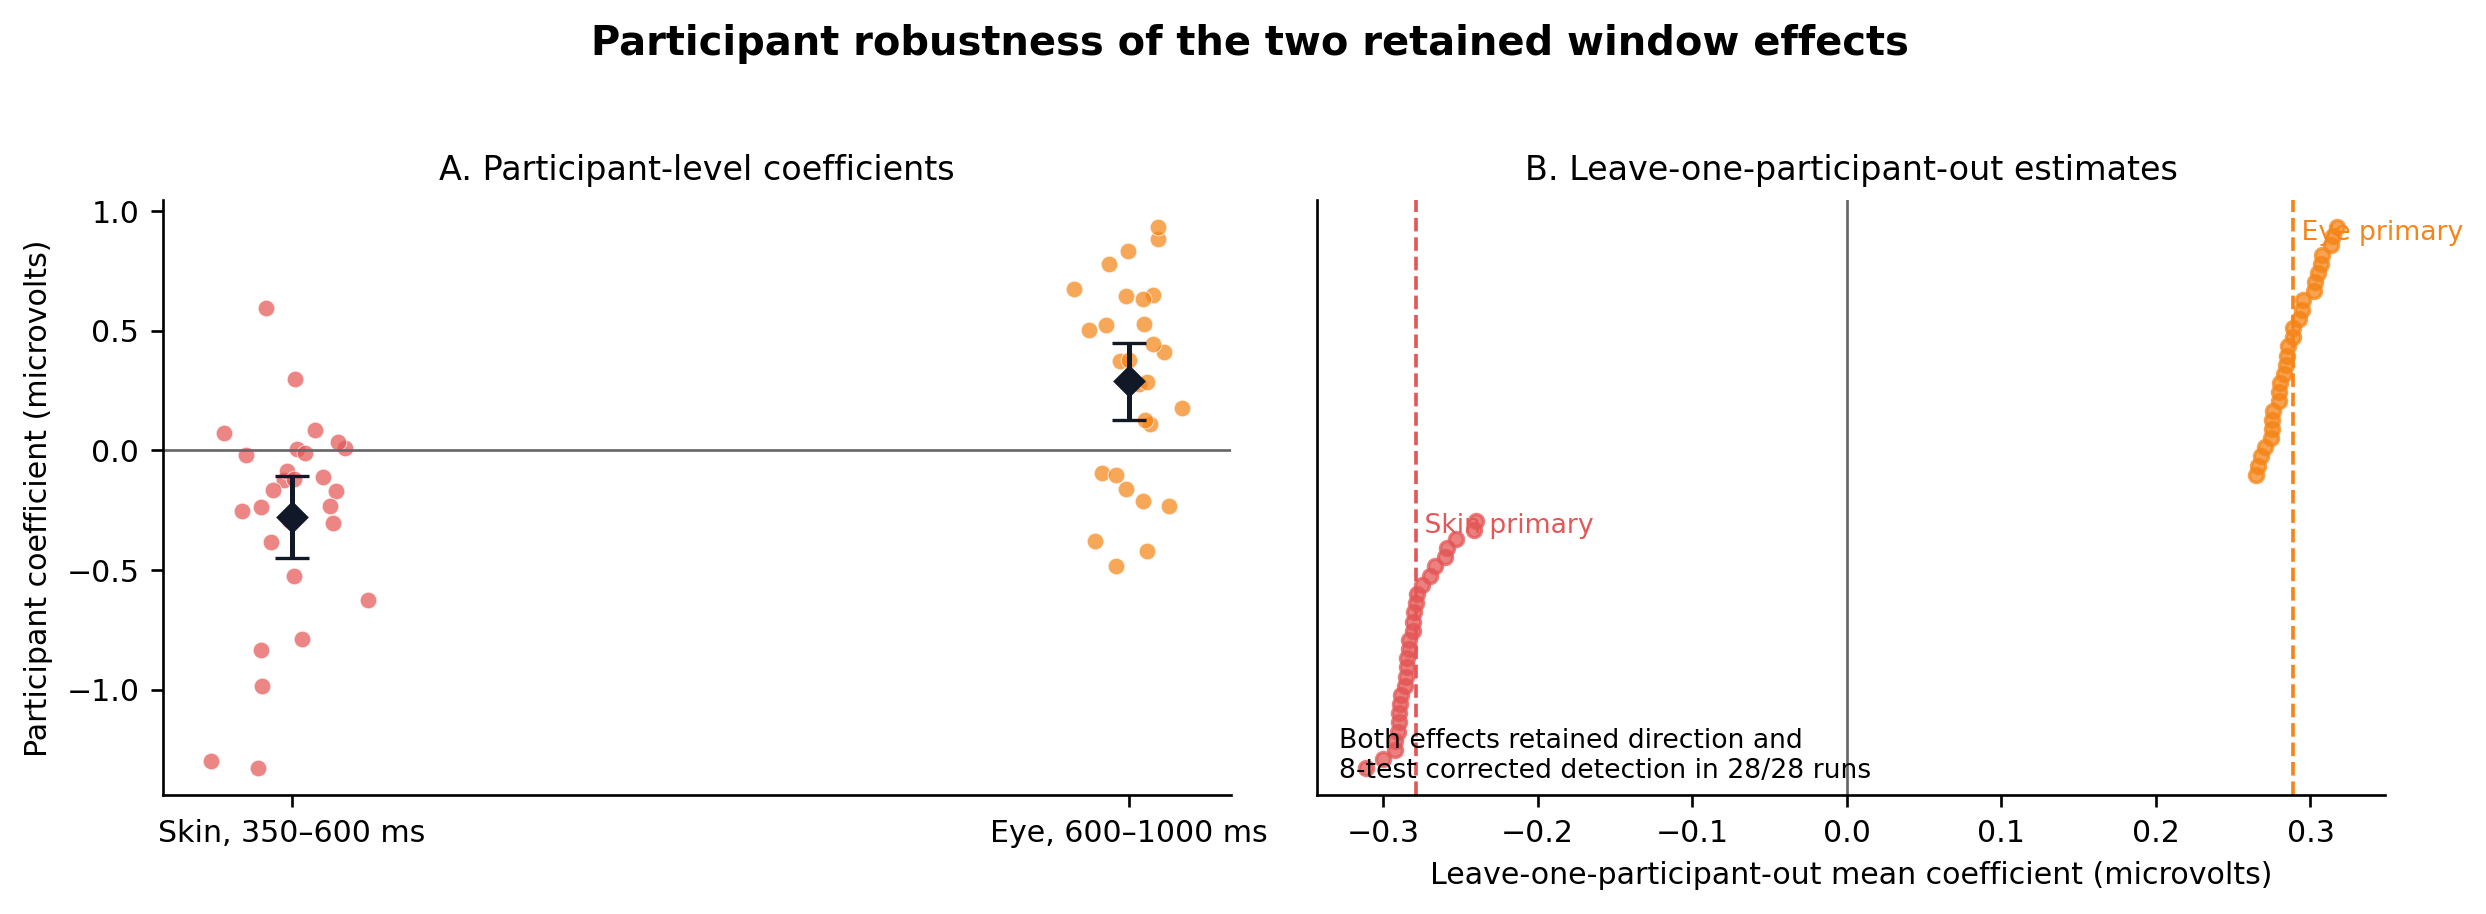
\includegraphics[width=\textwidth]{figures/Figure_6_participant_robustness.png}
\caption{参与者层稳健性。A：28名参与者的Skin 350--600 ms和Eye 600--1000 ms系数；B：28次留一参与者估计及主样本估计。两项效应在28/28版本中保持方向并通过同一8项校正。}
\label{fig:participantrobustness}
\end{figure}

\subsection{完整时程与跨层零结果}

完整0--1000 ms分析将四个操作和Surface-minus-Structural同时纳入五信号$\times$时间最大簇校正，没有簇达到$p<.05$。最接近门槛的是Surface-minus-Structural 420--580 ms（$\pfwe=.0513$）和Skin 440--580 ms（$\pfwe=.0808$）。因此，窗口结果不能用于声称精确、稳定的效应起止时间。

\begin{figure}[H]
\centering
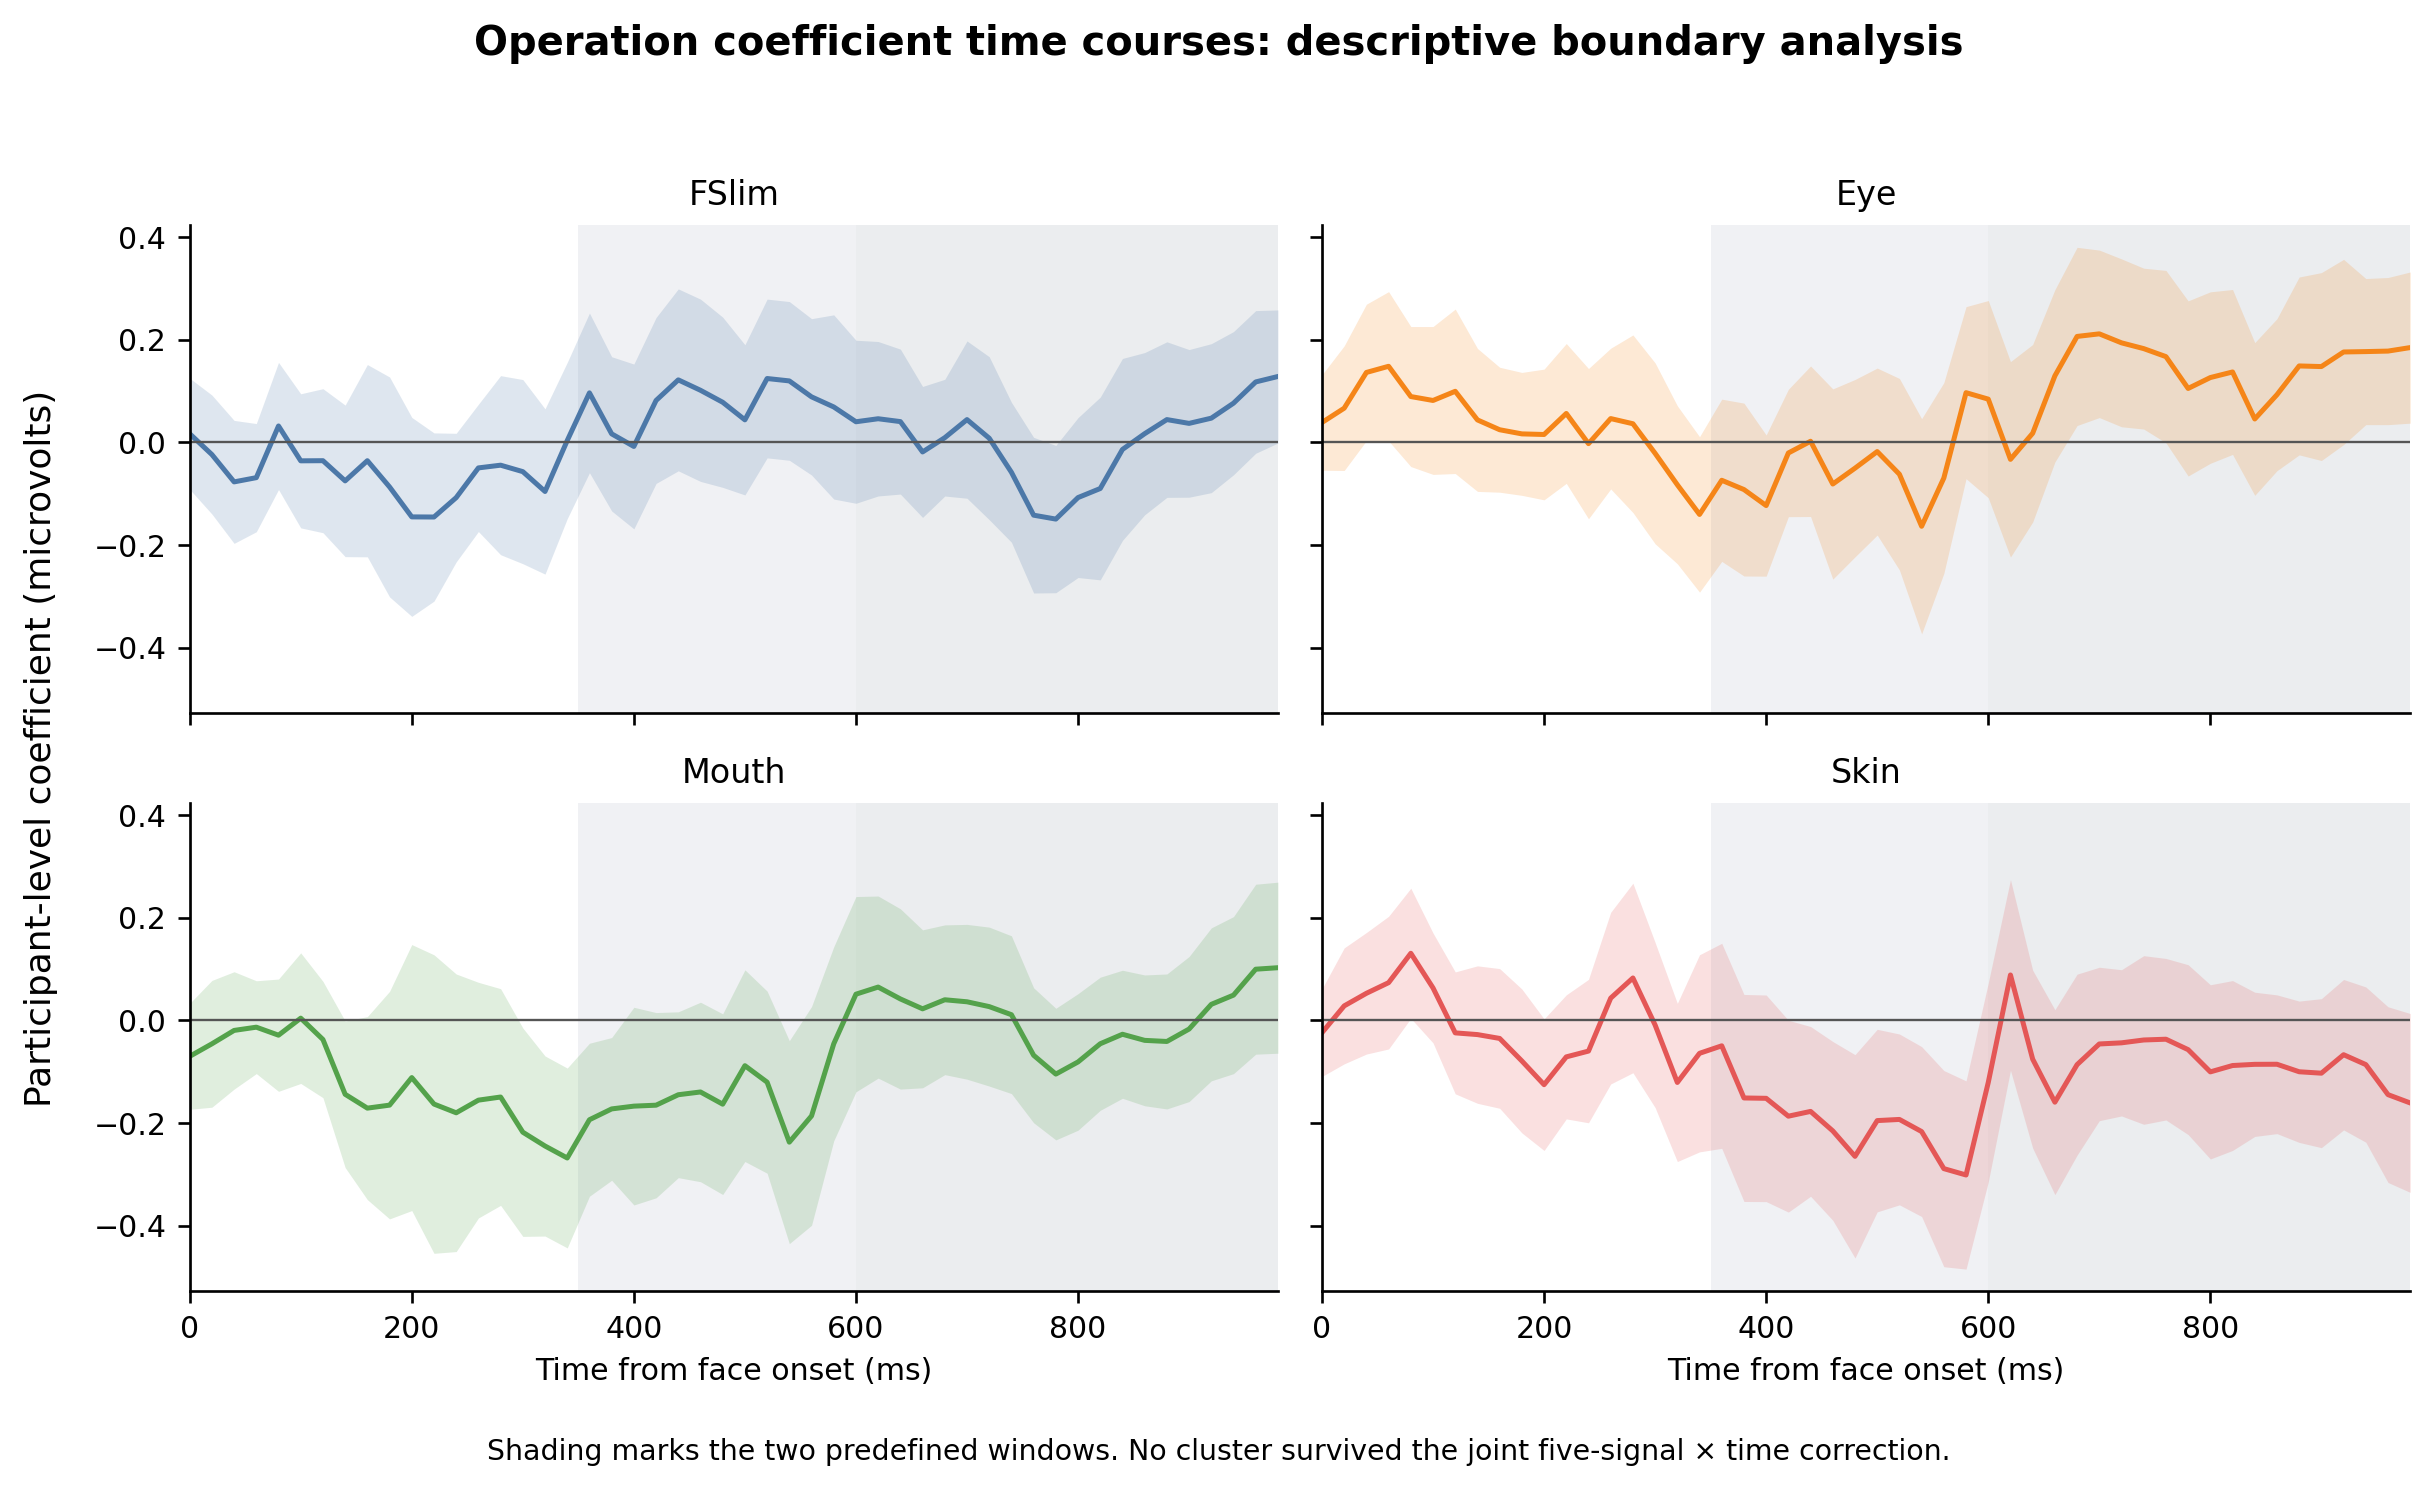
\includegraphics[width=\textwidth]{figures/Figure_5_full_timecourse_boundary.png}
\caption{四类操作的0--1000 ms参与者层描述性系数时程。阴影为95\%置信区间，灰色区域标出两个锁定窗口。该图用于显示整体时间形态；五信号$\times$时间联合簇校正没有显著簇，故不据此定义精确起止时间。}
\label{fig:timecourse}
\end{figure}

冻结A2在28人$G_{new}$/A2/$I\times$时间联合模型中没有显著簇，因而没有连续局部表面变化被EEG稳定追踪的证据。参与者层操作ERP系数与行为系数之间没有关联通过完整检验族校正；在嵌套留一参与者预测中加入ERP也没有优于只含编辑操作的模型，Beauty和Naturalness的平均MAE均略有恶化。补充边界审计还显示MVPA、RSA和$G_{new}$复现均未达到各自预设的保留门槛，因而不进入主文解释路线。

\section{讨论}

\subsection{主要发现：互补信息而非单一距离}

本研究得到三项相互制约的经验结果。第一，事后开发但在本次关联检验前锁定的A2主要反映当前刺激集中的双侧面颊表面变化，与几何错位、$G_{new}$及身份距离基本区分；它在变换溯源标签之外对未见参与者评价提供了小幅增量。第二，Skin与Eye分别在锁定的350--600 ms和600--1000 ms中央--顶叶窗口产生经过8项familywise校正的电位差异；两项结果不依赖单一参与者，并在四种身份遗漏版本中保持方向。第三，连续A2 EEG、EEG--评价个体关联和EEG评分增量预测均未获支持。数据因而支持输出状态与变换溯源的互补记录，不支持从计算指标经神经活动到评价的统一级联。

这一结果说明，信息表征的内容决定它可以回答什么。A2保留同一操作在不同图像上造成的实际局部表面差异；操作标签则保留编辑活动、受影响区域与来源语义。二者有关联但不能替代：前者没有稳定的连续EEG对应，后者却呈现条件相关的时间窗口差异。把二者压缩为一个“美化强度”会丢失这种互补性，而把它们排列成高低层级也会错误暗示其中一种可以包含另一种。

\subsection{Skin与Eye所在的时间加工范围}

Skin条件在350--600 ms中央--顶叶区域首先表现为负向平均电压差异。该窗口位于文献常讨论的后知觉中晚期评价范围，因此可以进一步提出一种谨慎解释：Skin操作可能伴随表面信息整合、编辑后一致性比较或评价更新。当前证据不能把该差异直接命名为N400，也不能把负向电压等同于审美冲突或不自然性感知，因为没有独立峰值、成分拓扑或构念特异性验证。

Eye条件在600--1000 ms表现为正向平均电压差异，其时间和极性与持续注意、评价精加工或反应准备等晚期活动相容，也可描述为late-positive或LPP-like差异\citep{Revers2023,Han2022}。这仍不是对经典LPP或唯一心理来源的确认；稳妥结论只是Eye操作在该预定时间范围内与中央--顶叶正向电位差异相关。

完整时程联合检验没有显著簇，因而350 ms和600 ms不是数据估计出的阶段边界。正确表述是：Skin和Eye条件差异分别位于既有文献所描述的中晚期与晚期范围，为操作敏感的时间定位提供条件性证据；早期效应、精确起止时间和早--中--晚序列均未在当前研究中得到支持。

\subsection{如何连接EEG与评价：条件层面趋同而非中介}

Skin和Eye操作在评价与EEG中都呈现条件差异，这构成\emph{条件层面趋同}：同一实验操纵影响两个测量模态。然而，两种效应的个体幅度没有可靠协变，EEG也没有改善未见参与者的评分预测。因此，趋同只能表示“操作$\rightarrow$评价”和“操作$\rightarrow$EEG”两条并列的条件关联，不能升级为“操作$\rightarrow$EEG$\rightarrow$评价”的中介或因果路径。

该边界对信息研究很重要：群体条件差异不能自动转化为个体差异解释，时间敏感信号也不必然成为有用的评价预测特征。EEG在本文中的贡献是限定人类加工发生差异的时间范围并排除过强路径，而不是提高系统预测性能。

\subsection{对信息处理与管理研究的贡献}

第一项贡献是表征原则：算法化视觉输出至少应同时保留\emph{输出状态信息}和\emph{变换溯源信息}。单一视觉距离只能回答最终状态的一部分，不能恢复生成该状态的操作、区域或强度。第二项贡献是评价原则：构念效度、样本外信息效用和时间对应必须分别检验。A2具有合理构念效度，样本内似然比也极显著，但参与者外$\Delta R^2$只有$.0211$；这正说明统计可检测性不等于高信息效用\citep{Shmueli2010,WangStrong1996}。同样，操作有时间窗口差异也不意味着EEG能够解释或预测评价。

在应用层面，最终图像的可审计元数据至少可以并列保存：（1）可复现的局部表面变化幅度；（2）编辑操作；（3）受影响区域；（4）参数或强度；以及（5）生成输出与原始实体之间的来源关系。这种记录方式与数据溯源和系统文档化原则一致\citep{MoreauMissier2013,Mitchell2019,Gebru2021}，并能避免在只剩最终图片时把结果状态误当作生成过程。不过，本研究没有测试真实平台中的选择、分享、信任、推荐效果或使用行为，不能声称上述记录会直接改善这些结果。

统一EEG样本、固定指标、联合多重校正、留一参与者与身份遗漏分析，是限制结果选择空间的方法强项。相应地，MVPA、RSA、连续EEG和G复现的未通过结果用于说明证据边界，而不是构造额外贡献。鉴于这些窗口是在Stage 2后锁定、并非前瞻性预注册，本文所有实证解释仍属探索性和刺激集受限。

\subsection{局限性与未来研究}

首先，研究只有4个基础身份。留一身份方向一致降低了单一刺激反转的担忧，但无法支持新身份或新刺激总体泛化。9,626个EEG试次提高的是参与者内系数精度，不会把4个身份变成数千个独立刺激。未来研究需要在更多身份、不同人口特征和独立编辑工具中预注册复现。

其次，EEG预处理流程只达到协议层面的可报告性。CleanLine和坏道处理分支不能逐参与者完全确认，完整的成分与epoch拒绝编号也没有保存。更严格的复现需要从Curry原始数据在版本锁定环境中重建，逐人记录坏道、ICA秩、ICLabel概率、拒绝成分和epoch，并与现有导数进行一致性比较。

第三，完整时程联合簇检验未显著，350 ms和600 ms不能被视为数据证明的阶段边界。未来独立样本应预注册ROI、窗口、效应方向和完整检验族，并直接比较潜伏期或成分拓扑。

第四，A2的参与者外增量较小，且只能代表双侧面颊区域的色彩、亮度和纹理变化，不构成通用视觉质量指标。G复现不足也说明landmark实现、标准化和成分定义需要更严格的版本管理。最后，当前脑--行为关联和增量预测为零；未来若要检验中介或级联，需要独立样本、明确时序模型、单试次关联以及预先规定的验证门槛，而不能在现有数据中继续搜索有利时间窗。

\section{结论}

在当前四身份刺激集中，双侧面颊局部表面变化A2在编辑操作之外对Beauty和Naturalness评价提供了有限的未见参与者增量信息；Skin和Eye操作则分别与350--600 ms负向和600--1000 ms正向中央--顶叶电位差异相关。两项EEG结果经过8项familywise校正、不依赖单一参与者，并在身份遗漏分析中保持方向。连续A2 EEG、EEG--评价关联和神经增量预测均未得到支持。算法化面部编辑因此更适合用输出状态与变换溯源两类互补信息来表征；当前证据是条件性、刺激集受限且增量价值有限的，不支持通用神经级联或跨身份泛化。

\section*{数据与代码可用性}

\todo{根据最终共享范围填写。建议说明派生统计表、审计文件和分析脚本的可用方式，并单独说明原始人脸图像及参与者EEG受到同意范围、隐私和图像许可限制。}

\section*{利益冲突}

\todo{作者声明。}

\section*{作者贡献}

\todo{按CRediT分类填写。}

\section*{生成式人工智能使用声明}

\todo{按Elsevier投稿时的最新政策和实际使用情况填写。}

\bibliographystyle{elsarticle-harv}
\bibliography{references}

\end{document}
